\chapter{Evaluation}\label{evaluation}
The purpose of this chapter was to explain how the final iteration of the prototype was evaluated. The evaluation aims to present the findings of the target group test, and provide a better understanding of, if the physical prototype facilitates collaboration in groups.\\

The final test was conducted on a 4th grade class at Skt. Annæ Skole  which was the same class, which the workshop (see \autoref{sec:workshop}) was conducted on. The goal of the test was to gather both quantitative data as well as qualitative data concerning the facilitation of collaboration. To do this, the test was divided into two separate parts. The qualitative part was an observational test, where the participants, within groups, performed a given task with the tool, which will be explained later in this chapter. The quantitative part was in the form of a Likert scale, concerning the experience of use of the tool in a collaborative manner. 

\section{The Test}
The test was conducted on 25 students divided into 5 groups, each group consisted of 5 students. Each group had an approximate 10-13 minutes for the first part of the test, and then 3-5 minutes filling out the Likert scale.

\subsection{The Setup} \label{setuptest}
At Skt. Annæ Skole, the first part of the test was conducted in an isolated room, and the second part right outside the room. Both environments were isolated from the rest of the class, as the testing of one group of participants took place, while the rest of the children were in their classroom having a lecture. The setup for the test can be seen in \autoref{fig:testSetupFinal}.\\

When the participating group were led into the room for the first part of the test, they were given a short introduction by the moderator, on how the prototype functions (with explicit attention to the areas of problem found in the usability test \autoref{improvementsUsability}). Afterwards, the participants were given the task to re-create the melody \textit{Mary Had a Little Lamb}, on the prototype. While playing the tune, the participants were being observed by two observers using the non-participant method\cite[p.~64-67]{bjoernerBog}.\\\\
When the participants completed the task, they were taken outside to complete a Likert scale about their collaboration using the prototype. To moderate this part of the test, a Likert scale moderator was used. The roles and their placement in relation to the participants, can be seen in \autoref{fig:testSetupFinal}.

\begin{figure}[H]
	\centering
	\includegraphics[width=0.7\linewidth]{figure/Evaluation/testSetupPlan.png}
	\caption{Figure shows the setup for the test. Top part of the figure shows the first part of the test. The bottom part shows the second part of the test.}
	\label{fig:testSetupFinal}
\end{figure} 


\subsubsection*{Moderator}
As stated above, the role of the moderator was to introduce the use and functions of the tool, as well as introduce the participants to the task that they were to perform. Furthermore, the moderator would answer any general questions, or questions regarding the execution of the task, such as usability questions. The moderator must however, not interfere with the execution of the task, to avoid causing biased participants\cite{bjoernerBog}. The moderator also had to make sure that the test was conducted according to plan, and that the task did not exceed the time limit.

\subsubsection*{Observers}
The observers would sit in the back of the room while not talking or interacting with the test participants in any way. They used the non-participant method, which means that they are not allowed to take any participation in the test.\\\\
When the test participants entered the room, they were each given a label on their shirt with an ID in form of a letter and a number, for the observers to keep track of the different participants. The labels were setup as "Group number"/"Letter", i.e. 1A, 1B, 1C, 1D, 1E, 2A, 2B, etc. The observers goal was to see if the test participants worked in a collaborative sense while testing the prototype. They would observe factors such as group roles, if a natural leader would take place or everyone attempted to work together equally etc. Furthermore, the observers would strive to observe which type of collaboration, or indications of same, would take place. 

\subsubsection*{Likert Scale moderator}
The Likert scale moderator would hand out papers with the Likert scale on, and introduce each question. As the participants were children, the moderators made sure to thoroughly explain each question and the possible answers to it, as well as answer the participants questions if they had any. The moderator would make sure that they did not induce bias the participants, by presenting both positive and negative answers equally. The moderator would also have the responsibility of noting the ID of the participants, on the related Likert scale paper. This was done in order to compare the data from the observation with the Likert scale data.

\subsection{The Likert scale setup}
The Likert scale was, as stated, used to measure whether the participants found the prototype collaborative or not, and to what extend. The questions focused on statements which would give insight, into how the test participant experienced the prototype, in relation to collaboration with the other participants. The purpose of the Likert scale was for the participants to answer both positively as well as negatively driven statements about different parts of collaboration i.e. if they felt that a person had more control than the others, or if they felt that they took part in the activities on the prototype. The 5 point scale ranged from \textit{Strongly Disagree} to \textit{Strongly Agree}. All the questions can be found below, the positively worded are colored with blue and the negatively worded questions are colored with red. For the exact Likert scale given to the participants, see appendices \ref{fig:likertScale} and \ref{sec:testPaper}.\\

\begin{enumerate}
	\item  \textcolor{blue}{I felt included in the use of the mat.}
	\item  \textcolor{blue}{I felt that the group worked together.}
	\item  \textcolor{red}{I did not feel that it was a group activity.}
	\item  \textcolor{blue}{I felt that i took part in making decisions.}
	\item  \textcolor{blue}{I felt that everybody took part in solving the tasks.}
	\item  \textcolor{blue}{I felt that we helped each other solve the tasks.}
	\item  \textcolor{blue}{I felt that some decided more than others.}
	\item  \textcolor{red}{I did not feel that i took part in deciding anything.}\\
\end{enumerate}
To evaluate and analyze the Likert scale data, different mathematical formulas were applied. To analyze the data, the mean was calculated, as well as the standard deviation to see how the responses turned out. To test the internal consistency of the test, the Cronbach's $\alpha$ formula was be applied (see \autoref{sec:cronbachAlpha}).


\section{Results}
In this section, the data gathered from the test will be presented and analyzed. The data from the Likert scale which will be presented in the following sections.

\subsection{Likert Scale}
To collect and gather all the data from the Likert scale, all the individual answers from the forms were put into a Matlab\footnote{https://matlab.mathworks.com/} script. Then, the data were put into a boxplot as seen in \autoref{fig:boxploteval}. As seen in the boxplot, the top of the blue square shows the third quartile, while the bottom shows the first quartile. The whiskers shows the maximum and minimum of the data. The red line on each question shows the median, so in question 1, the median is 4.\\
Looking at the figure, it is apparent that all questions except question 3 and 8 leans towards the Agreeing side. The reason for this is that question 3 and 8 is negatively worded question, which means that getting a negative answer can be flipped and then compared to the positive answers.

\begin{figure}[H]
	% This file was created by matlab2tikz.
%
%The latest updates can be retrieved from
%  http://www.mathworks.com/matlabcentral/fileexchange/22022-matlab2tikz-matlab2tikz
%where you can also make suggestions and rate matlab2tikz.
%
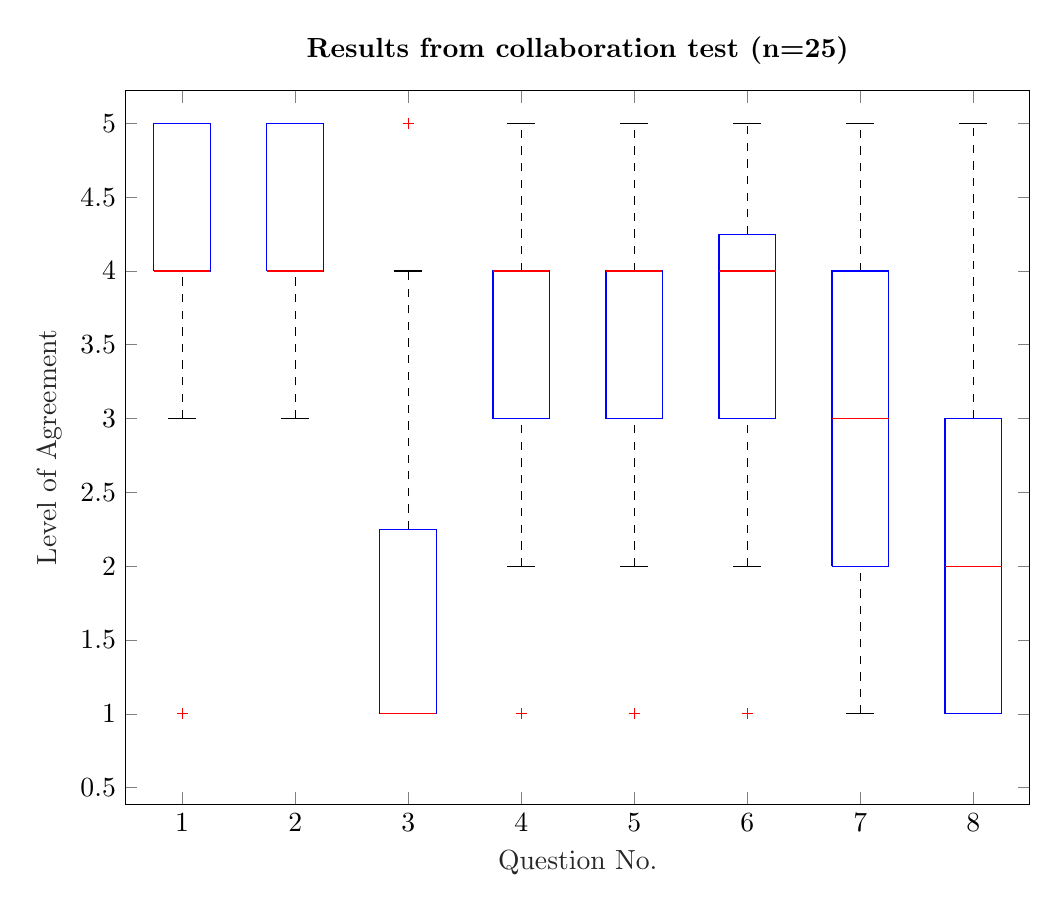
\begin{tikzpicture}

\begin{axis}[%
width=4.521in,
height=3.566in,
at={(0.758in,0.481in)},
scale only axis,
unbounded coords=jump,
xmin=0.5,
xmax=8.5,
xtick={1,2,3,4,5,6,7,8},
xlabel style={font=\color{white!15!black}},
xlabel={Question No.},
ymin=0.387875,
ymax=5.219625,
ylabel style={font=\color{white!15!black}},
ylabel={Level of Agreement},
axis background/.style={fill=white},
title style={font=\bfseries},
title={Results from collaboration test (n=25)},
legend style={legend cell align=left, align=left, draw=white!15!black}
]
\addplot [color=black, dashed, forget plot]
  table[row sep=crcr]{%
1	5\\
1	5\\
};
\addplot [color=black, dashed, forget plot]
  table[row sep=crcr]{%
2	5\\
2	5\\
};
\addplot [color=black, dashed, forget plot]
  table[row sep=crcr]{%
3	2.25\\
3	4\\
};
\addplot [color=black, dashed, forget plot]
  table[row sep=crcr]{%
4	4\\
4	5\\
};
\addplot [color=black, dashed, forget plot]
  table[row sep=crcr]{%
5	4\\
5	5\\
};
\addplot [color=black, dashed, forget plot]
  table[row sep=crcr]{%
6	4.25\\
6	5\\
};
\addplot [color=black, dashed, forget plot]
  table[row sep=crcr]{%
7	4\\
7	5\\
};
\addplot [color=black, dashed, forget plot]
  table[row sep=crcr]{%
8	3\\
8	5\\
};
\addplot [color=black, dashed, forget plot]
  table[row sep=crcr]{%
1	3\\
1	4\\
};
\addplot [color=black, dashed, forget plot]
  table[row sep=crcr]{%
2	3\\
2	4\\
};
\addplot [color=black, dashed, forget plot]
  table[row sep=crcr]{%
3	1\\
3	1\\
};
\addplot [color=black, dashed, forget plot]
  table[row sep=crcr]{%
4	2\\
4	3\\
};
\addplot [color=black, dashed, forget plot]
  table[row sep=crcr]{%
5	2\\
5	3\\
};
\addplot [color=black, dashed, forget plot]
  table[row sep=crcr]{%
6	2\\
6	3\\
};
\addplot [color=black, dashed, forget plot]
  table[row sep=crcr]{%
7	1\\
7	2\\
};
\addplot [color=black, dashed, forget plot]
  table[row sep=crcr]{%
8	1\\
8	1\\
};
\addplot [color=black, forget plot]
  table[row sep=crcr]{%
0.875	5\\
1.125	5\\
};
\addplot [color=black, forget plot]
  table[row sep=crcr]{%
1.875	5\\
2.125	5\\
};
\addplot [color=black, forget plot]
  table[row sep=crcr]{%
2.875	4\\
3.125	4\\
};
\addplot [color=black, forget plot]
  table[row sep=crcr]{%
3.875	5\\
4.125	5\\
};
\addplot [color=black, forget plot]
  table[row sep=crcr]{%
4.875	5\\
5.125	5\\
};
\addplot [color=black, forget plot]
  table[row sep=crcr]{%
5.875	5\\
6.125	5\\
};
\addplot [color=black, forget plot]
  table[row sep=crcr]{%
6.875	5\\
7.125	5\\
};
\addplot [color=black, forget plot]
  table[row sep=crcr]{%
7.875	5\\
8.125	5\\
};
\addplot [color=black, forget plot]
  table[row sep=crcr]{%
0.875	3\\
1.125	3\\
};
\addplot [color=black, forget plot]
  table[row sep=crcr]{%
1.875	3\\
2.125	3\\
};
\addplot [color=black, forget plot]
  table[row sep=crcr]{%
2.875	1\\
3.125	1\\
};
\addplot [color=black, forget plot]
  table[row sep=crcr]{%
3.875	2\\
4.125	2\\
};
\addplot [color=black, forget plot]
  table[row sep=crcr]{%
4.875	2\\
5.125	2\\
};
\addplot [color=black, forget plot]
  table[row sep=crcr]{%
5.875	2\\
6.125	2\\
};
\addplot [color=black, forget plot]
  table[row sep=crcr]{%
6.875	1\\
7.125	1\\
};
\addplot [color=black, forget plot]
  table[row sep=crcr]{%
7.875	1\\
8.125	1\\
};
\addplot [color=blue, forget plot]
  table[row sep=crcr]{%
0.75	4\\
0.75	5\\
1.25	5\\
1.25	4\\
0.75	4\\
};
\addplot [color=blue, forget plot]
  table[row sep=crcr]{%
1.75	4\\
1.75	5\\
2.25	5\\
2.25	4\\
1.75	4\\
};
\addplot [color=blue, forget plot]
  table[row sep=crcr]{%
2.75	1\\
2.75	2.25\\
3.25	2.25\\
3.25	1\\
2.75	1\\
};
\addplot [color=blue, forget plot]
  table[row sep=crcr]{%
3.75	3\\
3.75	4\\
4.25	4\\
4.25	3\\
3.75	3\\
};
\addplot [color=blue, forget plot]
  table[row sep=crcr]{%
4.75	3\\
4.75	4\\
5.25	4\\
5.25	3\\
4.75	3\\
};
\addplot [color=blue, forget plot]
  table[row sep=crcr]{%
5.75	3\\
5.75	4.25\\
6.25	4.25\\
6.25	3\\
5.75	3\\
};
\addplot [color=blue, forget plot]
  table[row sep=crcr]{%
6.75	2\\
6.75	4\\
7.25	4\\
7.25	2\\
6.75	2\\
};
\addplot [color=blue, forget plot]
  table[row sep=crcr]{%
7.75	1\\
7.75	3\\
8.25	3\\
8.25	1\\
7.75	1\\
};
\addplot [color=red, forget plot]
  table[row sep=crcr]{%
0.75	4\\
1.25	4\\
};
\addplot [color=red, forget plot]
  table[row sep=crcr]{%
1.75	4\\
2.25	4\\
};
\addplot [color=red, forget plot]
  table[row sep=crcr]{%
2.75	1\\
3.25	1\\
};
\addplot [color=red, forget plot]
  table[row sep=crcr]{%
3.75	4\\
4.25	4\\
};
\addplot [color=red, forget plot]
  table[row sep=crcr]{%
4.75	4\\
5.25	4\\
};
\addplot [color=red, forget plot]
  table[row sep=crcr]{%
5.75	4\\
6.25	4\\
};
\addplot [color=red, forget plot]
  table[row sep=crcr]{%
6.75	3\\
7.25	3\\
};
\addplot [color=red, forget plot]
  table[row sep=crcr]{%
7.75	2\\
8.25	2\\
};
\addplot [color=black, draw=none, mark=+, mark options={solid, red}, forget plot]
  table[row sep=crcr]{%
1	1\\
};
\addplot [color=black, draw=none, mark=+, mark options={solid, red}, forget plot]
  table[row sep=crcr]{%
nan	nan\\
};
\addplot [color=black, draw=none, mark=+, mark options={solid, red}, forget plot]
  table[row sep=crcr]{%
3	5\\
};
\addplot [color=black, draw=none, mark=+, mark options={solid, red}, forget plot]
  table[row sep=crcr]{%
4	1\\
};
\addplot [color=black, draw=none, mark=+, mark options={solid, red}, forget plot]
  table[row sep=crcr]{%
5	1\\
};
\addplot [color=black, draw=none, mark=+, mark options={solid, red}, forget plot]
  table[row sep=crcr]{%
6	1\\
};
\addplot [color=black, draw=none, mark=+, mark options={solid, red}, forget plot]
  table[row sep=crcr]{%
nan	nan\\
};
\addplot [color=black, draw=none, mark=+, mark options={solid, red}, forget plot]
  table[row sep=crcr]{%
nan	nan\\
};
\end{axis}
\end{tikzpicture}%
	\centering
	\caption{A boxplot showing all answers to each question from the Likert scale. The blue boxes represent the first and third quartile of the answers, the red lines represent the median, and the red dots represents the outliers which is in general disregarded.}
	\label{fig:boxploteval}
\end{figure}

To get a better understanding of the reliability of the test and the Likert items, the results were calculated with different formulas. In \autoref{fig:stddev} the mean of each question as well as the standard deviation were calculated. The reason that these were calculated, was to get insight in how much the responses deviated from each other. In the \autoref{fig:stddev}, the blue boxes shows the mean for each question and the whiskers how high the standard deviation is for each question. The standard deviation differs from question to question, but is approximately 1 in total.
\begin{figure}[H]
	% This file was created by matlab2tikz.
%
%The latest updates can be retrieved from
%  http://www.mathworks.com/matlabcentral/fileexchange/22022-matlab2tikz-matlab2tikz
%where you can also make suggestions and rate matlab2tikz.
%
\definecolor{mycolor1}{rgb}{0.00000,0.44700,0.74100}%
\definecolor{mycolor2}{rgb}{0.85000,0.32500,0.09800}%
%
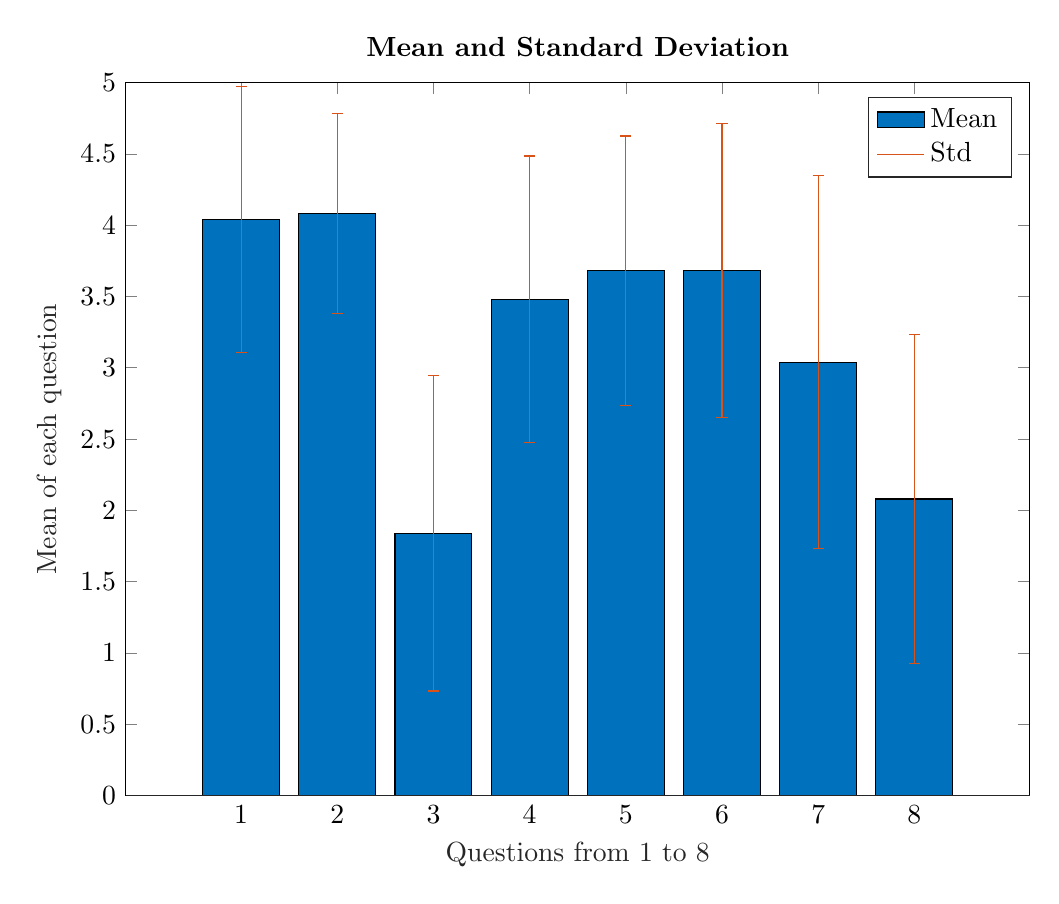
\begin{tikzpicture}

\begin{axis}[%
width=4.521in,
height=3.566in,
at={(0.758in,0.481in)},
scale only axis,
bar shift auto,
xmin=-0.2,
xmax=9.2,
xtick={1, 2, 3, 4, 5, 6, 7, 8},
xlabel style={font=\color{white!15!black}},
xlabel={Questions from 1 to 8},
ymin=0,
ymax=5,
ylabel style={font=\color{white!15!black}},
ylabel={Mean of each question},
axis background/.style={fill=white},
title style={font=\bfseries},
title={Mean and Standard Deviation},
legend style={legend cell align=left, align=left, draw=white!15!black}
]
\addplot[ybar, bar width=0.8, fill=mycolor1, draw=black, area legend] table[row sep=crcr] {%
1	4.04\\
2	4.08\\
3	1.84\\
4	3.48\\
5	3.68\\
6	3.68\\
7	3.04\\
8	2.08\\
};
\addplot[forget plot, color=white!15!black] table[row sep=crcr] {%
-0.2	0\\
9.2	0\\
};
\addlegendentry{Mean}

\addplot [color=mycolor2, draw=none]
 plot [error bars/.cd, y dir = both, y explicit]
 table[row sep=crcr, y error plus index=2, y error minus index=3]{%
1	4.04	0.934523051258413	0.934523051258413\\
2	4.08	0.702376916856849	0.702376916856849\\
3	1.84	1.1060440015358	1.1060440015358\\
4	3.48	1.00498756211209	1.00498756211209\\
5	3.68	0.945163125250522	0.945163125250522\\
6	3.68	1.0295630140987	1.0295630140987\\
7	3.04	1.30639452948436	1.30639452948436\\
8	2.08	1.15181016954473	1.15181016954473\\
};
\addlegendentry{Std}

\end{axis}
\end{tikzpicture}%
	\centering
	\caption{This figure displays the mean plotted in bars marked with blue, and the standard deviation as the error bars marked with red}
	\label{fig:stddev}
\end{figure}



Furthermore, the mean and the standard deviation for each question can be seen in \autoref{table:questionsCalc}. This table also displays the measured Cronbach's $\alpha$ of the Likert scale. The Cronbach's $\alpha$ results in a total of 0.56, which is in general considered lower than acceptable, a rule of thumb is that 0.7 or above is the acceptable (see \autoref{sec:cronbachAlpha}). 

\begin{table}[H]
\centering
\caption{The results from the calculating the mean, variance and standard deviation on each question's responses (N=25).}
\label{table:questionsCalc}
\begin{tabular}{@{}cccclc@{}}
\toprule
\multicolumn{1}{l}{Question} & \multicolumn{1}{l}{Mean} & \multicolumn{1}{l}{Variance} & \multicolumn{1}{l}{Std} &  & \multicolumn{1}{l}{Cronbach's $\alpha$} \\ \midrule
1                            & 4.040                    & 0.8733                       & 0.934                   &  & 0.392                              \\
2                            & 4.080                    & 0.493                        & 0.702                   &  & 0.530                              \\
3                            & 4.160                    & 1.223                        & 1.106                   &  & 0.552                              \\
4                            & 3.480                    & 1.010                        & 1.004                   &  & 0.464                              \\
5                            & 3.680                    & 0.893                        & 0.945                   &  & 0.443                              \\
6                            & 3.680                    & 1.060                        & 1.029                   &  & 0.434                              \\
7                            & 3.040                    & 1.7067                       & 1.306                   &  & 0.807                              \\
8                            & 3.920                    & 1.326                        & 1.151                   &  & 0.412                              \\ \midrule
Overall                        & \multicolumn{1}{l}{}     & \multicolumn{1}{l}{}         & \multicolumn{1}{l}{}    &  & 0.5682                             \\ \bottomrule
\end{tabular}
\end{table}

\subsection{Observation Test}
For the observational part of the test, the two observers wrote down the activities of each group, how they collaborated, and any miscellaneous things of interest. The condensed version of these notes can be seen in \autoref{table:observationalNotes}, while the full version of the notes can be found in appendix \autoref{table:observationalNotesBig}. 
\begin{table}[H]
\centering
\caption{Table showing the condensed version of the observational notes from the test}
\label{table:observationalNotes}
\resizebox{\textwidth}{!}{%
\begin{tabular}{@{}ccccc@{}}
\toprule
Group 1 & Group 2 & Group 3 & Group 4 & Group 5 \\ \midrule
C natural leader & Chaotic & \begin{tabular}[c]{@{}c@{}}A, B, E tries to\\ guide other members\end{tabular} & No natural leader & \begin{tabular}[c]{@{}c@{}}B reluctant leader\\ guiding the others\end{tabular} \\
\begin{tabular}[c]{@{}c@{}}Other members try\\ to instruct each other\end{tabular} & Disorganised & C is passive in background & \begin{tabular}[c]{@{}c@{}}Guiding each other\\ interchangeably\end{tabular} & \begin{tabular}[c]{@{}c@{}}D tries to assist in\\ guidance\end{tabular}\\ 
E controls the box & E controls the box & \begin{tabular}[c]{@{}c@{}}D elected to contol the box\\Later A takes over\end{tabular} & B controls the box & E controls the box \\ \midrule

\bottomrule
\end{tabular}%
}
\end{table}
As for collaboration, group 1 and group 5 mostly had a natural leader, while group 3 and group 4 had a more dynamic leadership, with either three or more \textit{"leaders"} guiding the group. No natural group leader was observed to occur within group 2, and the group's collaboration was noted to be chaotic and disorganized.